\documentclass[tikz,border=2pt,11pt]{standalone}
\usetikzlibrary{arrows.meta}
\usetikzlibrary{patterns}
\usetikzlibrary{calc}
\usetikzlibrary{positioning}
\usepackage{amsmath}
\usepackage{amssymb}
\usepackage{tikz}
\newcommand{\Z}{\mathbb Z}
\newcommand{\R}{\mathbb R}
\newcommand{\C}{\mathbb C}
\newcommand{\N}{\mathbb N}
\newcommand{\E}{\mathbb E}
\newcommand{\1}{\mathbf 1}
\newcommand{\dd}{\,\mathrm d}
\newcommand{\abs}[1]{\lvert #1\rvert}
\newcommand{\norm}[1]{\lVert #1\rVert}
\newcommand{\ip}[2]{\langle #1,#2\rangle}
\DeclareMathOperator{\dist}{dist}
\DeclareMathOperator{\supp}{supp}
\DeclareMathOperator{\Tr}{Tr}
\begin{document}
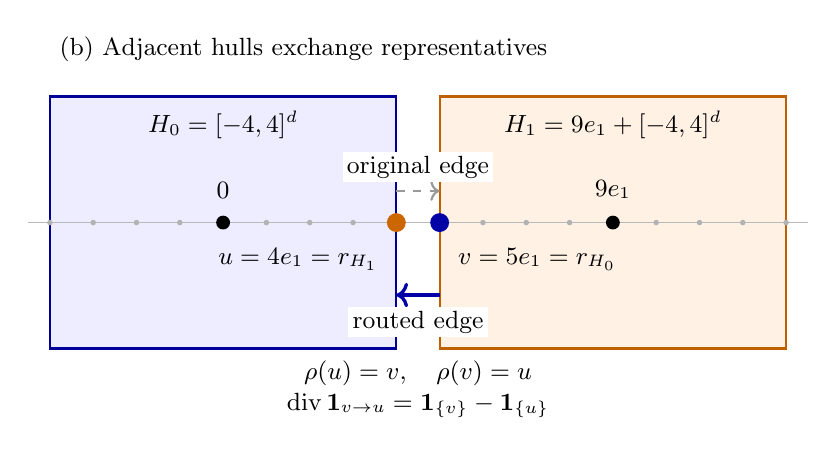
\begin{tikzpicture}[x=.55cm,y=.4cm,font=\small]
  \node[anchor=west] at (-4,5.5)
    {(b) Adjacent hulls exchange representatives};
  \fill[blue!7] (-4,-4) rectangle (4,4);
  \draw[blue!60!black,thick] (-4,-4) rectangle (4,4);
  \fill[orange!10] (5,-4) rectangle (13,4);
  \draw[orange!75!black,thick] (5,-4) rectangle (13,4);
  \draw[gray!55] (-4.5,0)--(13.5,0);
  \foreach \x in {-4,...,13} {\fill[gray!60] (\x,0) circle (1pt);}
  \fill (0,0) circle (2.5pt);
  \fill (9,0) circle (2.5pt);
  \node[above=5pt] at (0,0) {$0$};
  \node[above=5pt] at (9,0) {$9e_1$};
  \node at (0,3.1) {$H_0=[-4,4]^d$};
  \node at (9,3.1) {$H_1=9e_1+[-4,4]^d$};
  \draw[fill=white,blue!65!black,thick] (5,0) circle (3pt);
  \draw[fill=white,orange!80!black,thick] (4,0) circle (3pt);
  \node[anchor=north east] at (3.8,-.5) {$u=4e_1=r_{H_1}$};
  \node[anchor=north west] at (5.2,-.5) {$v=5e_1=r_{H_0}$};
  \draw[->,gray!80,dashed,thick] (4,1)--(5,1);
  \node[above=3pt,fill=white,inner sep=1.5pt] at (4.5,1) {original edge};
  \draw[->,blue!65!black,very thick] (5,-2.3)--(4,-2.3);
  \node[below=4pt,fill=white,inner sep=1.5pt] at (4.5,-2.3) {routed edge};
  \node[align=center] at (4.5,-5.3)
    {$\rho(u)=v,\quad\rho(v)=u$
     \\ $\operatorname{div}\1_{v\to u}=\1_{\{v\}}-\1_{\{u\}}$};
\end{tikzpicture}
\end{document}
